\documentclass[paper=a4, twocolumn, fontsize=10pt]{article} % A4 paper and 11pt font size
\usepackage{graphicx,float,subfig}
\usepackage[english]{babel} % English language/hyphenation
\usepackage{amsmath,amsfonts,amsthm,tensor} % Math packages
\usepackage[shortlabels]{enumitem} 
\usepackage{sectsty} % Allows customizing section commands



\allsectionsfont{\centering \normalfont\scshape} % Make all sections centered, the default font and small caps

\numberwithin{equation}{section} % Number equations within sections
\numberwithin{figure}{section} % Number figures within sections 
\numberwithin{table}{section} % Number tables within sections 
\setlength\parindent{0pt} % Removes all indentation from paragraphs 

\newcommand{\horrule}[1]{\rule{\linewidth}{#1}} % Create horizontal rule command with 1 argument of height

\title{	
\normalfont \normalsize 
\horrule{.5pt}\\ % horizontal rule
\Large Circuit EOM's \\ 
\horrule{1pt}\\ % horizontal rule
}
\author{}
\date{\normalsize}%\today}



\def\ket#1{\left\vert #1 \right\rangle}
\def\bra#1{\left\langle #1 \right\vert}
\def\ip#1#2{\left\langle #1 \vert #2 \right\rangle}
\def\opex#1#2#3{\left\langle#1\left\vert#2\right\vert#3\right\rangle}
\def\deriv#1 #2{\frac{\text{d}}{\text{d}#2} #1}
\def\fderiv#1#2{\frac{\dd#1}{\dd#2}}
\def\pderiv#1#2{\frac{\partial}{\partial #2} #1}
\def\npderiv#1 #2 #3{\frac{\partial^#1}{\partial #3^#1} #2}
\def\fpderiv#1 #2{\frac{\partial #1}{\partial #2} }
\def\fnpderiv#1 #2 #3{\frac{\partial^#1 #2}{\partial #3^#1}}
\def\fnderiv#1 #2 #3{\frac{\dd^#1 #2}{\dd #3^#1}}
\def\B#1{\textbf{#1}}
\def\cross {\times}
\def\tbf #1{\textbf{#1} }
\def\det {\text{Det}}
\def\comm#1,#2.{\left[ #1,#2\right]}
\def\tr {\text{Tr}}
\def\dd{\text{d}}
\def\at#1{\Big{|}_{#1}}

\def \df#1{\hat{#1}}

\graphicspath{{./img/}}
\begin{document} 

\maketitle % Print the title

\section{superconducting loops and the josephson equations}

Let's start with a few assumptions that we wont investigate in detail:

One will be the cooper pair macroscopic wavefunction:
$\psi = \sqrt{\rho} e^{i\varphi}$. Here, we have considered that a large number of charge carries have condensed into the same state and that $|\psi|^2$ gives the density of these charge carriers. Notably, this gives us an expression for the electirc current density, since it s proportional to the probability current density:
 \[ J = \frac{e}{m} \left( \frac{i\hbar}{2} \left(\psi\nabla\psi^* - \psi^*\nabla\psi\right) - 2e A |\psi|^2\right) \]


 note the charge is $2e$, while the charge to mass ratio is the same as a single electron because we are dealing with pairs of electrons.
\\
\subsection{josephson equations}
When we consider two superconductors "weakly linked" by a thin dialectric barrier, we can sort of treat them as a a single superconductor because $\varphi$ in one of the superconductors is not independent of the phase in the other). We assume each superconductor has a macroscoping wavefunction $\psi_{1,2} = \sqrt{\rho_{1,2}} e^{i\varphi_{1,2}}$ and write the hamiltonian over base states representing a particle in one superconductor or the other: $H =E_1 \ket{1}\bra{1} + E_2 \ket{2}\bra{2} + K \ket{1}\bra{2} + K \ket{2}\bra{1}$. A state vector in this basis is given by: $\ket{\psi} = \psi_1 \ket{1} + \psi_2\ket{2}$.  Setting $E_1 - E_2 = 2eV$, and using the shrodinger equation leads us to the josephson equations (I can expand on this if anyone is interested) for a junction where the potential across the junction is $V$:

\begin{align}
\label{jj_eq1}
    I = I_{c_1} \sin \varphi^*
    \\
\label{jj_eq2}
    \partial_t \varphi^* = \frac{2\pi V}{\Phi_0}
\end{align}
where $\varphi^* = \varphi_2 - \varphi_1$ and $\Phi_0$ is the flux quantum. When considering magnetic field effects, you must transform the expression above to be gauge invariant by 

\[ \varphi^* \to \varphi_J = \varphi^* -  \frac{2\pi}{\Phi_0} \int_{junction} A \cdot dl \]


\subsection{Fluxoid quantization}

Lets start by plugging the macroscopic wavefunction into the equation for the current density-- which gives us:

\[ J = \frac{\rho e}{m} \left(\hbar\nabla \varphi - 2e A \right) \]

which can be solved for the spatial derivative of the phase:

\[ \nabla \varphi = \frac{2\pi}{\Phi_0}  A + \alpha J  \]


First, we can get the gauge invariant variable $\varphi_J$ for the phase difference $\varphi$ by integrating across the junction and subtracting off the part that depends the vector potential ($\alpha$ is defined by context):

\begin{align}
    \varphi_J = \int_{junction} \nabla \varphi \cdot dl -  \frac{2\pi}{\Phi_0} \int_{junction} A \cdot dl
    \\
    = \varphi^* -  \frac{2\pi}{\Phi_0} \int_{junction} A \cdot dl
\end{align}

If we imagine a superconducting loop with a JJ interrupting it-- we can integrate around the loop to incorporate the phase chage across the junction into a quantization condition. Integrating around the whole loop gives

\[ \oint \nabla \varphi \cdot dl = 2\pi n\]

\begin{figure}[H]
    \centering
    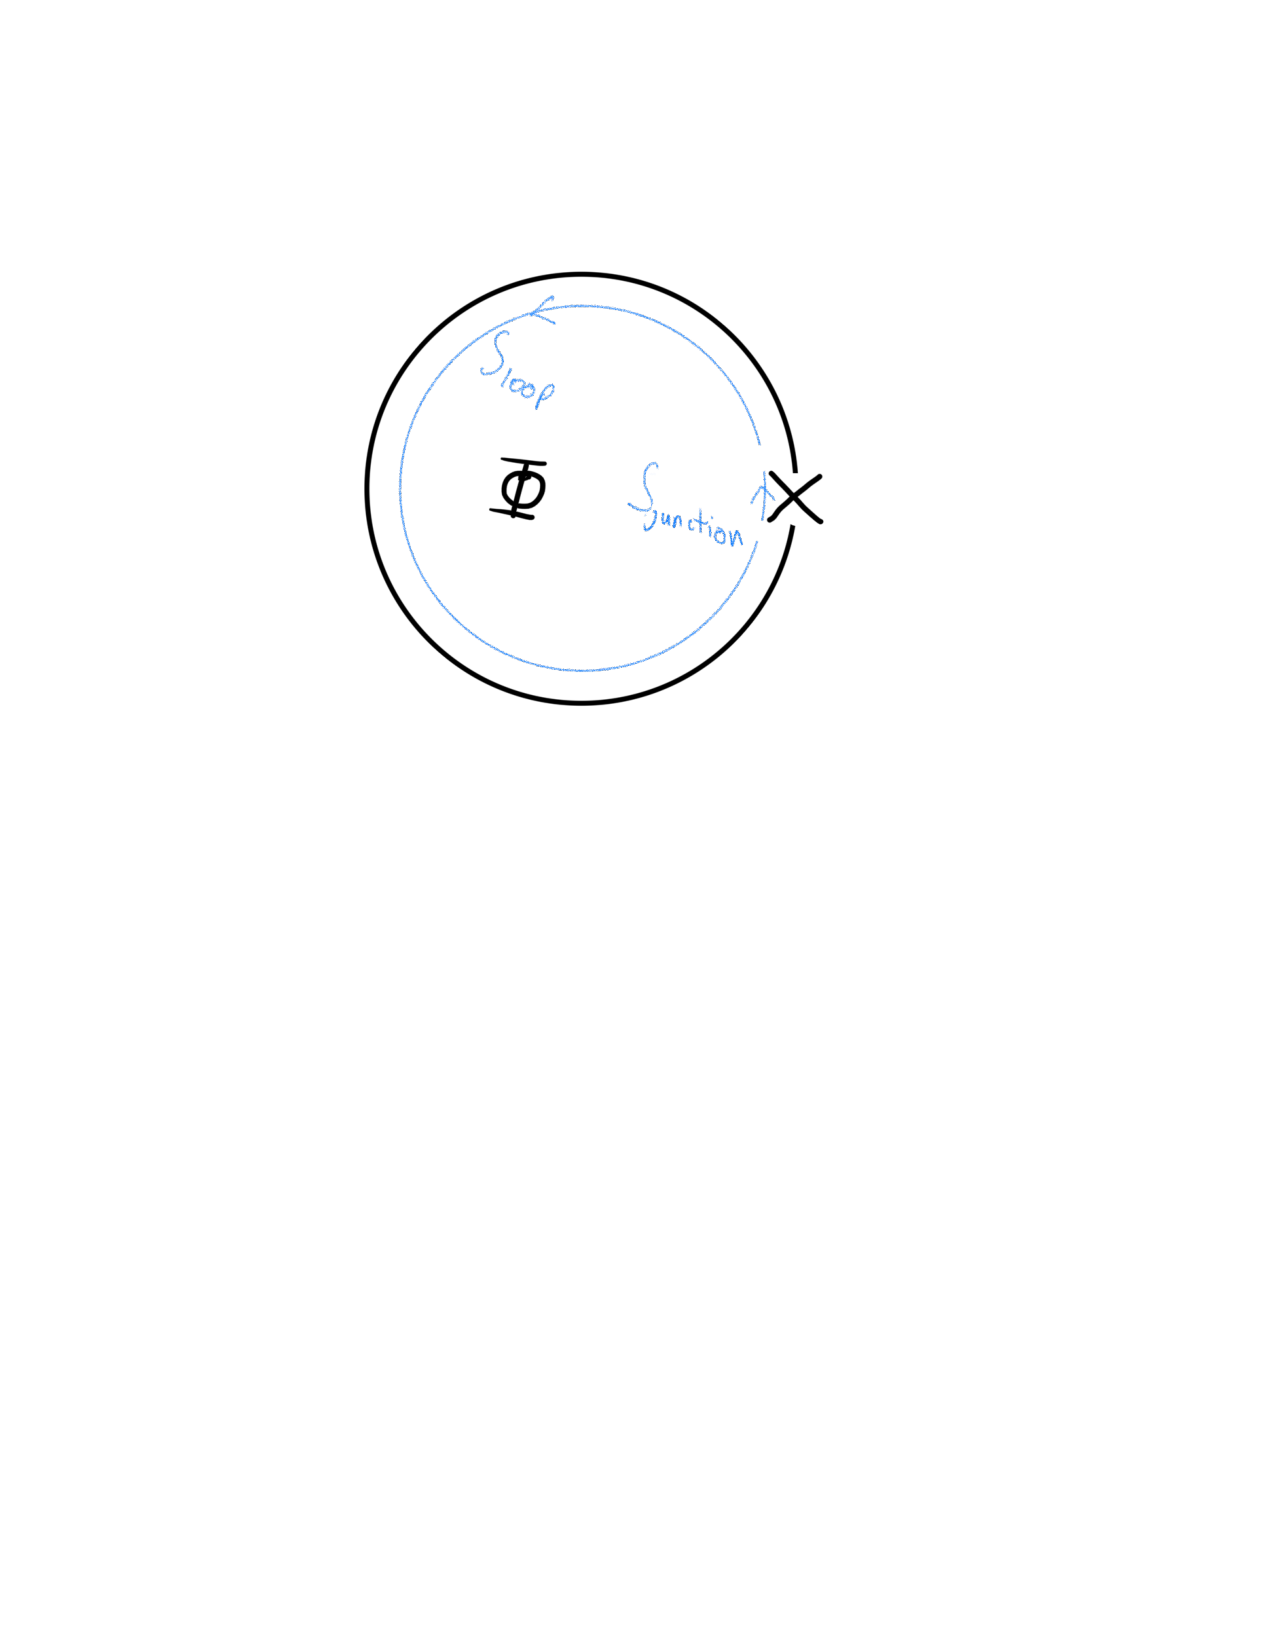
\includegraphics[scale=.5]{JJ_loop.pdf}
    \caption{ "loop" should be "wire"}
    \end{figure}

The above somes from a single-valuedness condition. If we integrate around the whole loop we should com back to where we started-- which means that wavefunction must have changed phase by a multiple of $2\pi$. Now, we can also decompose the integral into parts that are across the junction and parts that are in the superconducting wire:


\begin{align}
    2\pi n &= \varphi^* + \int_{wire} \nabla \varphi \cdot dl
    \\
    &= \varphi_J +  \frac{2\pi}{\Phi_0} \int_{junction} A  \cdot dl + \int_{wire} \nabla \varphi \cdot dl
    \\
    &= \varphi_J +  \frac{2\pi}{\Phi_0} \oint A  \cdot dl + \int_{wire} \alpha J  \cdot dl
\end{align}
where, the the last step, we have separated out the parts of the integration that depend on the vector potential and the parts that depend on the supercurrent density. Now, the integral in the superconducting loop can be taken to be zero as long as we can find a path where we travel inside of the penetration depth of the supercurrent (generally seems to be accepted as viable unless the superconducting wire is ultra thin). The vector potential term is nothing other than the magnetic flux threading the superconducting loop-- recognizing that $B = \nabla \times A$ and using green's theorem. This gives us the "fluxoid quantization condition":

\[ \varphi_J = 2\pi n - \frac{2\pi}{\Phi_0} \Phi \]

that relates the phase change inside of a JJ in a superconducting loop to the magnetic flux $\Phi$ that threads the loop. This can be extended to multiple junctions in the loop

\[ \sum_i \varphi_{J_i} = 2\pi n - \frac{2\pi}{\Phi_0} \Phi \]


\section{The EOM for the single DC/RF squid combo}

Using the tried and true method of finding circuit EOM, we will write out a bunch of equations and then solve them so find how manty degrees of freedom we have. The advantage of this is that it is straightforward, and easily interpreted. The downside is that as the circuit complexity grows, the degrees of freedom become more complicated.

A few important notes on the conventions I am going to use. First, it is useful to introduce dimensionless/dimensionful versions of phases/fluxes; that are related as: $ \df \theta \equiv  \frac{\Phi_0}{2\pi} \theta  $ where $\Phi_0$ is the flux quantum and $\theta$ is a dimensionless phase difference. This brings simplicity to the equations at the cost of having to remember that two variables relate to the same degree of freedom, and that $ \partial_{\df \theta} {\theta} = \frac{2\pi}{\Phi_0}$. An $``x"$ subscript on a variable denotes the externally applied fluxes that are typically thought of as our control parameters. It is important to conceptually distinguish $\df\theta$, for example, which would be the scaled version of the JJ phase difference $\theta$ with units of magnetic flux and  $\df\varphi_{xL}$ which would be an externally applied flux that has a dimensionless scaled version $\varphi_{xL}$. Finally, upper case $\Phi$ variables will refer to quantities that are proper magnetic fluxes for which we will not be interested in dimensionless versions.


For the DC/RF combo SQUID that was used in previous experiemnts (based off of the work done by Siyuan Han in the late 80s/early 90s), the process of finding the EOM is as follows:

First, we take the RSJ model for the JJ elements and write the currents passing through them-- Kirchoffs junction equations. (note the terms proportional to time derivatives of $\df \theta$ come from the second josephson equation $\partial_t \df \theta_i =  V_i $ ):

\begin{align}
    I_3 = I_{c_1} \sin \theta_1 + \frac{C}{2} \ddot{\df \theta}_1 + \frac{1}{R} \dot{ \df \theta }_1
    \\ 
    I_4 = I_{c_2} \sin \theta_2 + \frac{C}{2} \ddot{\df \theta}_2 + \frac{1}{R} \dot{ \df \theta}_2
    \end{align}
From here on out, we are going to supress the dissipative term proportional to $R$-- as it will just travel around with the capacitive term. We will just remeber that each "acceleration" term is going to come with a dissipative term proportional to $\frac{1}{R}$.

Now, we will relate the fluxes threading the different loops to the phases across each JJ using fluxoid quantization:

\begin{align}
     n_L\Phi_0 - \Phi_L = -\df\theta_1
    \\ 
    n_R \Phi_0 -  \Phi_R = \df\theta_2
    \\
    n_C \Phi_0 - \Phi_{C} = \df\theta_1  - \df\theta_2
\end{align}

where $\Phi_L, \Phi_R, \Phi_{C}$ are the fluxes threading the three loops in the circuit diagram. We choose all $n=0$. This conceptually represents something like a ground state assumption, but I do not think any of the arguments in this writeup depend on this choice. To see this, note that the way an integral multiple of $2\pi$ enters Eq. \ref{jj_eq1} and \ref{jj_eq2} yileds them invariant to $n$. Meanwhile, the total fluxes are given by the sum of all sources of fluxes in the corresponding loop: namely the self inductances and external fluxes.

\begin{figure}[H]
\centering
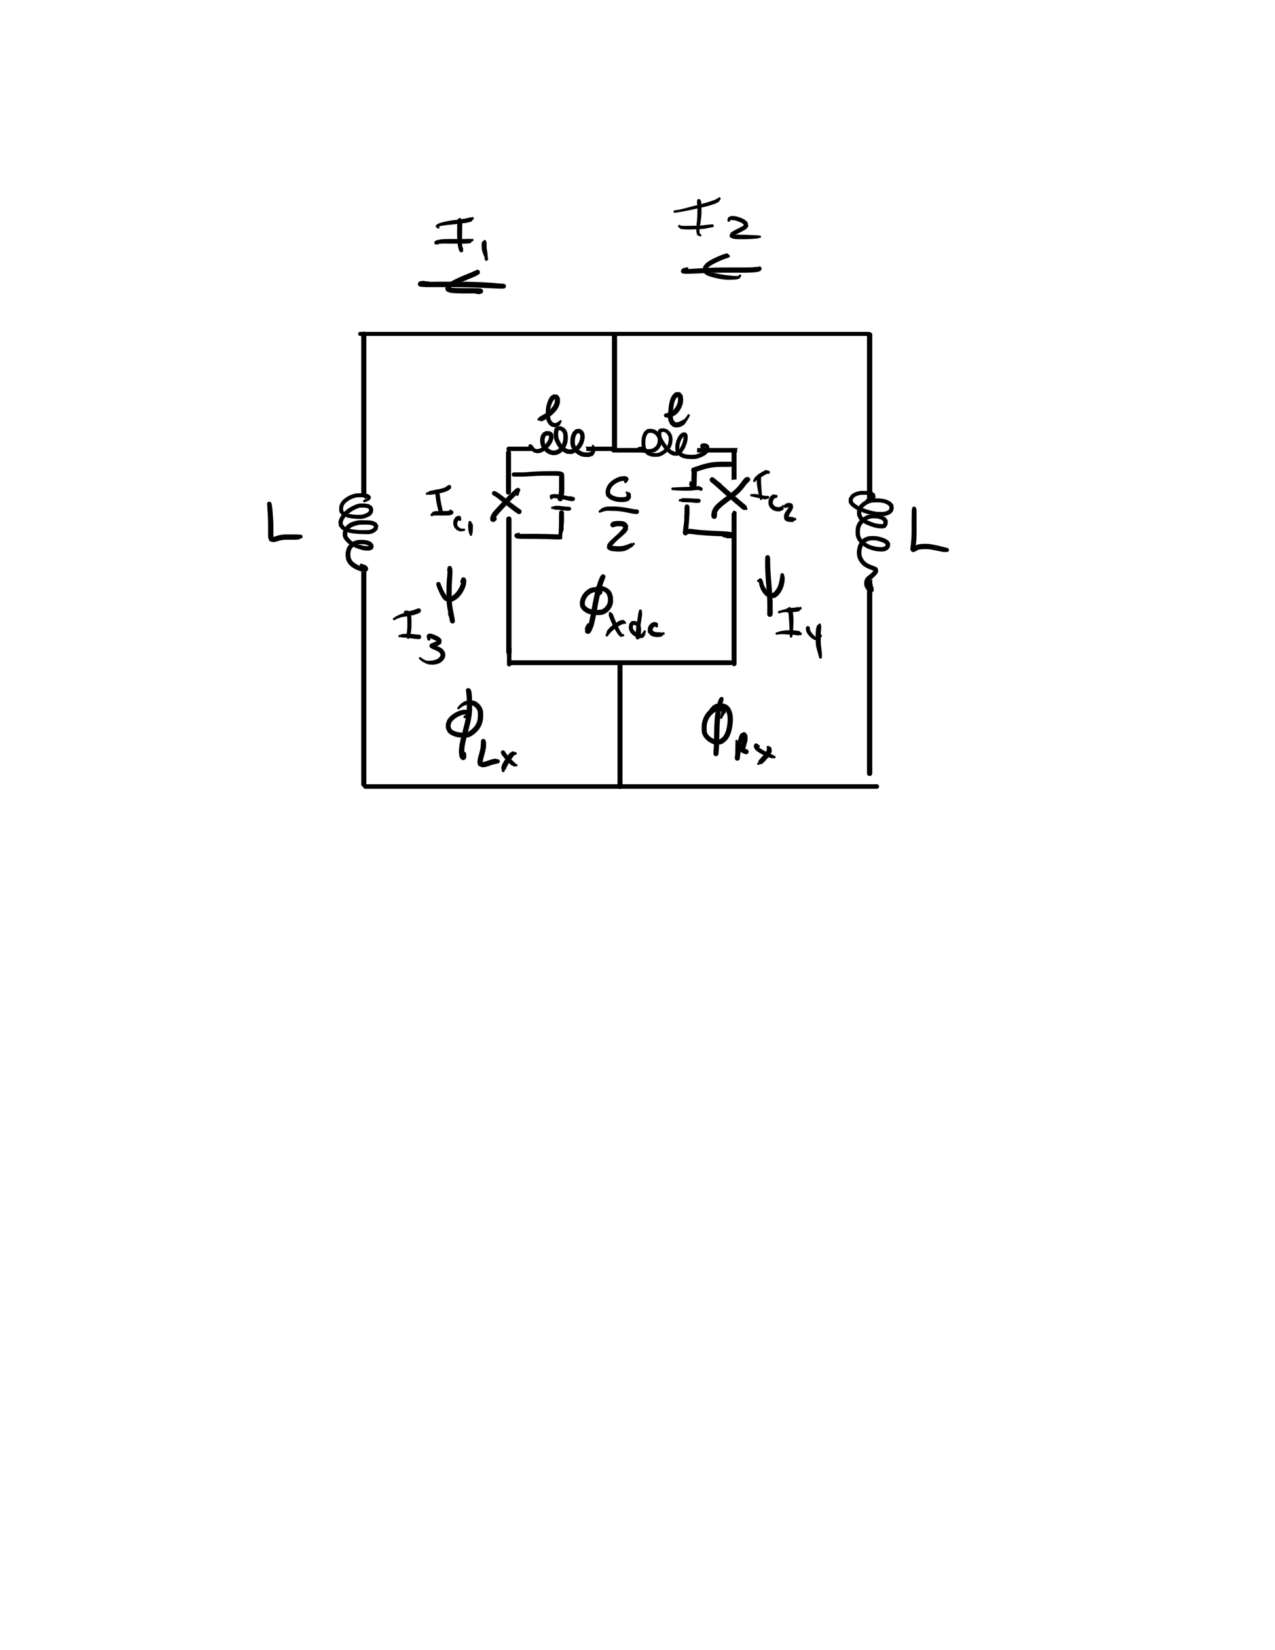
\includegraphics[scale=.5]{circuit_diagram.pdf}
\caption{I have made notation changes not reflected in the diagram. $L \to \tilde{L}; \phi_{xL} \to \df\varphi_{xL}; \phi_{xR} \to \df\varphi_{xR};  \phi_{xdc} \to \df\varphi_{xdc}  $
}
\end{figure}

\begin{align}
    I_1 \tilde{L} - I_3 \ell + \df\varphi_{xL} = \Phi_{L} = \df\theta_1
    \\
    I_2 \tilde{L} + I_4 \ell + \df\varphi_{xR} = \Phi_{R} = -\df\theta_2
    \\
    I_3 \ell - I_4 \ell + \df\varphi_{xdc} = \Phi_{C} = -(\df\theta_1 - \df\theta_2)
\end{align} 

Now that we have the circuit equations, all thats left is algebra. It is important to note that we have defined 4 currents, but we actually have a relationship betweem them ($I_2 = I_1 + I_3 + I_4$) which suggests 3 variables should do the trick. With foresight towards where we want to end up, lets take some linear combinations of our junction equations:

\begin{align}
\frac{C}{2} (\ddot{\df\theta}_1 + \ddot{\df\theta}_2 ) = (I_3 + I_4) - I_{c_1} \sin \theta_1 - I_{c_2} \sin \theta_2
\\
\frac{C}{2} (\ddot{\df\theta}_2 - \ddot{\df\theta}_1 ) = (I_4 - I_3) +I_{c1} \sin\theta_1 - I_{c2} \sin \theta_2
\end{align}

We now eliminate the current terms by using the loop equations. Note that we can solve for $I_3+I_4$ by subtracting the first two loop equations because $I_2 - I_1 = I_3+I_4$. Combining the first tow loop equations yields:

\begin{align}
    I_3 + I_4 = \frac{1}{\ell+\tilde{L}}\left(- \df\theta_1 - \df\theta_2 - \df\varphi_{xR} + \df\varphi_{xL} \right)
    \\
    I_4 - I_3 =\frac{1}{\ell}\left( -\df\theta_2 + \df\theta_1 +\df\varphi_{xdc}\right)
    \end{align}


lets define $\df\varphi = \frac{1}{2}\left(\df\theta_1 + \df\theta_2\right)$ and $\df\varphi_{dc} = \df\theta_2 - \df\theta_1$ (equivalently we can think of defining the corresponding $\varphi$, and $\varphi_{dc}$ in terms of $\theta_1,\text{and } \theta_2$). Note, if we had chosen to set any of $n_L,n_R,n_C$ equal to anything other than zero, you would absorb them into these definitions, and then we don't worry about them anymore. We also set $\df\varphi_{xL} = -\df\varphi_{xR} = \df\varphi_x$, since we have the freedom to set our external fluxes to be whatever we want.

\begin{align}
    I_3 + I_4 = \frac{2}{\ell+\tilde{L}}\left(\df\varphi_x - \df\varphi \right)
    \\
    I_4 - I_3 =\frac{1}{\ell}\left(\df\varphi_{xdc} - \df\varphi_{dc} \right)
    \end{align}

Finally, we substitute into the junction equations to get:


\begin{align}
    C \ddot{\df\varphi} = \frac{2}{\ell+\tilde{L}}\left( \df\varphi_x - \df\varphi \right) - I_{c_1} \sin \theta_1 - I_{c_2} \sin \theta_2
    \\
    \frac{C}{2} \ddot{\df\varphi}_{dc}= \frac{1}{\ell}\left( \df\varphi_{xdc} -\df\varphi_{dc}\right) +I_{c1} \sin\theta_1 - I_{c2} \sin \theta_2
    \end{align}
With some new definitions of the constants from the PRR: $\tilde{L} = 2L-\ell$ and $\gamma = \frac{L}{2\ell}$ we have:

\begin{align}
    C \ddot{\df\varphi} = \frac{1}{L}\left( \df\varphi_x - \df\varphi \right) - I_{c_1} \sin \theta_1 - I_{c_2} \sin \theta_2
    \\
    \frac{C}{4} \ddot{\df\varphi}_{dc}= \frac{\gamma}{L}\left( \df\varphi_{xdc} -\df\varphi_{dc}\right) +\frac{1}{2}I_{c1} \sin\theta_1 - \frac{1}{2} I_{c2} \sin \theta_2
    \end{align}


Using the relations $\theta_1 = \varphi - \frac{1}{2}\varphi_{dc} $ and $\theta_2 = \varphi + \frac{1}{2}\varphi_{dc} $ we eliminate the $\theta_i$. We will also introduce $I_{\pm} \equiv I_{c2} \pm I_{c1}$.  This yields:

\begin{align}
    C \ddot{\df\varphi} &= \frac{1}{L}\left( \df\varphi_x - \df\varphi \right) - 
    \\
    &I_{+} \sin \varphi \cos \frac{\varphi_{dc}}{2} - I_{-} \cos \varphi \sin \frac{\varphi_{dc}}{2}
    \\
    \frac{C}{4} \ddot{\df\varphi}_{dc} &= \frac{\gamma}{L}\left( \df\varphi_{xdc} -\df\varphi_{dc}\right) - 
    \\
    &\frac{I_{+}}{2} \cos \varphi \sin \frac{\varphi_{dc}}{2} - \frac{I_{-}}{2} \sin \varphi \cos \frac{\varphi_{dc}}{2}
\end{align}

If we think about the equations as being the lagrangian EQOM of the system-- we have:

\begin{align}
C \ddot{\df\varphi} =- \partial_{\df\varphi} U(\df\varphi, \df\varphi_{dc})
\\
\frac{C}{4} \ddot{\df\varphi}_{dc} =  - \partial_{\df\varphi_{dc}} U(\df\varphi, \df\varphi_{dc})
\end{align}


Reintroducing the resistive shunt to the josephson elements, would result in term proportional to $\dot{\phi}$ or $\dot{\phi}_{dc}$, as below:

\begin{align}
C \ddot{\df\varphi} = \lambda \dot{\df\varphi} - \partial_{\df\varphi} U(\df\varphi, \df\varphi_{dc})
\\
\frac{C}{4} \ddot{\df\varphi}_{dc} = \lambda_{dc} \dot{\df\varphi}_{dc} - \partial_{\df\varphi_{dc}} U(\df\varphi, \df\varphi_{dc})
\end{align}

revealing the connection between the equations of motion above and the damping term in a Langevin equation. Thus, when simulating this circuit with thermal fluctuations, we use langevin dynamics. An equation of the form below:

\[ m d \dot{\df\varphi} = \lambda \dot{\df\varphi} dt - \partial_{\df\varphi} U(\df\varphi, \df\varphi_{dc}) dt + r(t) \sqrt{2 k_B T \lambda dt} \]

for each dimension-- where the effective damping coefficient and mass depend on the physical parameters $R,L,C$.
\\
\\
Now, to find the exact form for the potential-- which is useful for visualization purposes. We first verify wether we can think of these functions as having come from a potential at all-- because we know that for any function $\partial_{x} \partial_{y} U(x,y) = \partial_{y} \partial_{x} U(x,y)$; we verify that

\begin{align}
 \partial_{\df\varphi_{dc}}\left[I_{+} \sin \varphi \cos \frac{\varphi_{dc}}{2} + I_{-} \cos \varphi \sin \frac{\varphi_{dc}}{2}\right]
\end{align}
\[=\]
\begin{align} 
    \partial_{\df\varphi}\left[\frac{I_{+}}{2} \cos \varphi \sin \frac{\varphi_{dc}}{2} + \frac{I_{-}}{2} \sin \varphi \cos \frac{\varphi_{dc}}{2}\right]
\end{align}

The above hold true, so we have a physical potential. In fact, the potential is easy enough to be found by inspection: 
\begin{align}
U &= \frac{1}{2L} (\df\varphi-\df\varphi_x)^2 + \frac{\gamma}{2L} (\df\varphi_{dc}-\df\varphi_{xdc})^2 + \\
 &\frac{\Phi_0}{2\pi}  \left( - I_+ \cos \varphi \cos \frac{\varphi_{dc}}{2} + I_- \sin \varphi \sin \frac{\varphi_{dc}}{2}\right)
\end{align}

Finally, we can introduce the energy scale $U_0 = \frac{ \Phi_0^2}{4\pi^2 L} $, which allows us to write the potential as:

\begin{align}
    \frac{U}{U_0} \equiv V(\varphi, \varphi_{dc}) =  \frac{1}{2} (\varphi-\varphi_x)^2 + \frac{\gamma}{2} (\varphi_{dc}-\varphi_{xdc})^2
    \\
     - \beta \cos \varphi \cos \frac{\varphi_{dc}}{2} + \delta\beta \sin \varphi \sin \frac{\varphi_{dc}}{2}
    \\
\end{align}

where the $\beta,\delta\beta \equiv \frac{2\pi L}{\Phi_0} I_{\pm}$. Note that there is a difference between the epxression here and the potential in the PRR. This is because there is a $\pi$ phase shift in the definition of $\varphi$ depending on the reference ($\varphi \to \varphi-\pi$). This seems to be done more often in modern work, I belive it is because it sets $\varphi=0$ to be the center of a well. We can see that defining both $\varphi,\varphi_{x}$ to have a pahse shift of $\pi$ would lead our last two terms to switch signs. Interestingly, the PRR has a positive sign for both terms-- though I dont think it is particularly important since the $\delta\beta$ term doesnt have a particular reason to be positive or nagative-- it will depend on particular fabrication details-- and will need to be measured for a given device.

The potential given in the simulations is the one with the $\pi$-shifted definition of $\varphi$:

\begin{align}
    \frac{U}{U_0} \equiv V(\varphi, \varphi_{dc}) =  \frac{1}{2} (\varphi-\varphi_x)^2 + \frac{\gamma}{2} (\varphi_{dc}-\varphi_{xdc})^2
    \\
     + \beta \cos \varphi \cos \frac{\varphi_{dc}}{2} - \delta\beta \sin \varphi \sin \frac{\varphi_{dc}}{2}
    \\
\end{align}



 In this case, we were able to come up with a potential, but I want to note that it is not strictly necesarry to find the "potential" when the equations of motion are already known . Let's move on to find the EOM for some coupled devices.


\section{ RF-RF coupling}

Imagine two identical devices, each with it's own set of variables denoted from eachother with primes ($I_1'$, for example being the current in the second device along the same section as $I_1$ is in the first device). The absolute simplest coupling I can imagine is to couple the "rf" squid sections together with mutual inductances, $M, M'$. This changed our equations very little. The junction and fluxoid qunatization equations will not be changed at all, we still have equations, for example, the equations

\begin{align}
    I_3 = I_{c_1} \sin \theta_1 + \frac{C}{2} \ddot{\Phi}_1 + \frac{1}{R} \dot{\Phi}_1
    \\ 
    I_4 = I_{c_2} \sin \theta_2 + \frac{C}{2} \ddot{\Phi}_2 + \frac{1}{R} \dot{\Phi}_2
    \end{align} 
Again, we are going to supress the dissipative terms for now-- to simplify the algebra. Of course, note that we now have 2 sets of these: one for the original device and one for the "primed" one.  The flux threading each subloop loop will, however, see the addition of the mutual inductances between the two devices:

\begin{align}
    MI_1' + I_1 \tilde{L} - I_3 \ell + \phi_{Lx} = \Phi_{L} = \phi_1
    \\
    MI_2' + I_2 \tilde{L} + I_4 \ell + \phi_{Rx} = \Phi_{R} = -\phi_2
    \\
    I_3 \ell - I_4 \ell + \phi_{xdc} = \Phi_{C} = -(\phi_1 - \phi_2)
\end{align} 

We will have an analogous set of these for the primed device, where the mutual inductance $M'$ is coupled to the unprimed currents $I_1, I_2$. This coupling is particularly simple because of the symmetry between the two devices. It is straightforward to see how the same definitions of $\phi,\phi_{dc}$ (and $\phi',\phi_{dc}'$) Will lead to the following equation of motion for $\phi,\phi'$. Namely, when we solve for $I_3+I_4$ in each circuit using the equations above-- we get:

\[ I_3 + I_4 = \frac{2}{\ell+\tilde{L}}\left(\phi_x - \phi \right) - \frac{M}{\ell+\tilde{L}} (I_3'+I_4') \]

Which, when plugged into the junction equations, gives us:

\begin{multline}
    C \ddot{\phi} = \frac{2}{\ell+\tilde{L}}\left( \phi_x - \phi \right) - \frac{M}{\ell+\tilde{L}} (I_3'+I_4') \\ - I_{c_1} \sin \theta_1 - I_{c_2} \sin \theta_2
\end{multline}

(note that the $\phi_{dc}$ EOM is unchanged when compared to the uncoupled devices):

Remembering that we have another set of equation where the primes and unprimes are switched, we can substitute the primed versions of the junction equations into the EOM above:

\begin{multline}
    C \ddot{\phi} = \frac{2}{\ell+\tilde{L}}\left( \phi_x - \phi \right) \\ - \frac{M}{\ell+\tilde{L}} ( C\ddot{\phi}' + I_{c1}\sin \theta_1' + I_{c2} \sin \theta_2') \\ - I_{c_1} \sin \theta_1 - I_{c_2} \sin \theta_2
\end{multline}

This can be rearragned so that we have (note the reintroduction of $I_{\pm}$ as well as $L\to 2L-\ell$ and the definition $\mu\equiv \frac{M}{2L}$)

\begin{multline}
    C \left(\ddot{\phi}+ \mu \ddot{\phi}' \right) = \frac{1}{L}\left( \phi_x - \phi \right) -  \\
    I_{+} \sin \varphi \cos \frac{\varphi_{dc}}{2} - I_{-} \cos \varphi \sin \frac{\varphi_{dc}}{2} \\
    - \mu ( I_{+} \sin \varphi' \cos \frac{\varphi'_{dc}}{2} + I_{-} \cos \varphi' \sin \frac{\varphi'_{dc}}{2})
\end{multline}

and a similar EOM with permuted primes. Now, we can see that we are no longer in the normal coordiantes of the system, where we can look at the LHS of the equations as a partial derivative of a Lagrangian with respect to some canonical $\dot{x}$. In preparation of some algebra, lets write out our two EOM using the following definition:

\[ F(x,y) \equiv I_{+} \sin x \cos \frac{y}{2} + I_{-} \cos x \sin \frac{y}{2} \]

This yields:

\begin{align}
    C \left( \ddot{\phi} + \mu \ddot{\phi}'\right) = \frac{1}{L} (\phi_x-\phi) - F(\varphi, \varphi_{dc}) - \mu F(\varphi',\varphi_{dc}')
    \\
    C \left( \mu' \ddot{\phi} + \ddot{\phi}'\right) = \frac{1}{L} (\phi'_x-\phi') - F(\varphi', \varphi'_{dc}) - \mu' F(\varphi,\varphi_{dc})
\end{align}

Let's ignore the $F$ and constant part of the EOM for now, and work on diagonalizing the other part. As a vector equation, we have something like (here, and only here, $\phi = (\phi, \phi')$):

\begin{align}{
    C A \ddot{\mathbf{\phi}} = \frac{1}{L} \phi 
}
\end{align}
where $A = \begin{pmatrix} 1 & \mu \\ \mu' & 1 \end{pmatrix}  $ has eigenvectors/values:

\[  (-\sqrt\frac{\mu}{\mu'}, 1)/1-\sqrt{\mu\mu'}\]
 and 
 \[ (\sqrt\frac{\mu}{\mu'}, 1)/1+\sqrt{\mu\mu'}\]. 
 
 These eigenvectors are not orthogonal to each other, unless $\mu'=\mu$. We specialize to this case, which suggests new coordiantes $\eta = -\phi +\phi'$ and $\eta' = \phi+\phi'$ with associated $\eta_x = -\phi_x + \phi_x'$ and $\eta_x' = \phi_x + \phi_x'$ . The effective EOM of these composite degrees of freedom can be found by adding and subtracting the EOM above, this yields:

\begin{multline}
    C(1-\mu) \ddot{\eta} = \frac{1}{L} (\eta_x-\eta) - \\ F(\varphi', \varphi'_{dc}) - \mu F(\varphi,\varphi_{dc}) + F(\varphi, \varphi_{dc}) + \mu F(\varphi',\varphi_{dc}')
\end{multline}
    \\
\begin{multline}
    C(1+\mu) \ddot{\eta}' = \frac{1}{L} (\eta'_x-\eta') - \\ F(\varphi', \varphi'_{dc}) - \mu F(\varphi,\varphi_{dc}) - F(\varphi, \varphi_{dc}) - \mu F(\varphi',\varphi_{dc}')
\end{multline}

All of the coordiantes are linear combinations and/or scaled versions of each other, so we can also write $F$ in terms of the $\eta$'s. Before doing so, lets simplify the above a little: 

\begin{multline}
    C \ddot{\eta} = \frac{1}{L(1-\mu)} (\eta_x-\eta) + F(\varphi, \varphi_{dc}) - F(\varphi', \varphi'_{dc})
\end{multline}
    \\
\begin{multline}
    C \ddot{\eta}' = \frac{1}{L(1+\mu)} (\eta'_x-\eta') - F(\varphi, \varphi_{dc}) - F(\varphi', \varphi'_{dc})
\end{multline}

Again, we are interested in wether we can express the RHS of all of these EOM as the gradient of some potential function. We can check wether these force terms come from a potential energy function by checking

\[ \partial_{\eta'} \left( F(\varphi, \varphi_{dc}) - F(\varphi', \varphi'_{dc})\right) = \partial_{\eta} \left( -F(\varphi, \varphi_{dc}) - F(\varphi', \varphi'_{dc})\right) \]


Defining $\zeta,\zeta'$, nondimensional versions of $\eta,\eta'$, we have: $\varphi = \frac{1}{2} (-\zeta+\zeta')$ $\varphi' = \frac{1}{2} (\zeta+\zeta')$. This will allow us to check the relation above easily by noting that each of the four terms above will result in a string of partial derivatives like the one below

\[ \frac{\partial F(\varphi,\varphi_{dc})}{\partial \eta'}  =\frac{\partial \zeta'}{\partial \eta'} \frac{\partial \varphi}{\partial \zeta'} \frac{\partial F}{\partial \varphi} \]

will always take a similar form for every term. The first derivative will be common among all terms ($\frac{2\pi}{\Phi_0}$), and the second will be either $\pm \frac{1}{2}$ depending on if we are talking about primed or unprimed $\varphi$ and $\zeta$. Notating $f(x,y)$ as the derivative $\partial_x F(x,y)$ The result is:

\[ \frac{1}{2} f(\varphi, \varphi_{dc}) - \frac{1}{2} f(\varphi', \varphi'_{dc}) = - \left(-\frac{1}{2}\right) f(\varphi, \varphi_{dc}) - \frac{1}{2} f(\varphi', \varphi'_{dc})\]

Which suggests we might be abel to find a proper potential. If we want to consider the case where $\gamma$ is large, and the $dc$ coordinates stay close to the external fluxes-- then this is good enough. However, if we are goig to simulate the full dynamics including the $dc$ coordinates, we have some more work to do.

The EOM for $\phi_{dc}$ and $\phi_{dc}'$ are unchanged by the coupling. If we translate them into our current notation, we have:
\begin{align}
\frac{C}{2} \ddot{\phi}_{dc} &= \frac{2\gamma}{L}\left( \phi_{xdc} -\phi_{dc}\right) -  F(\frac{\varphi_{dc}}{2}, 2\varphi) \\
\frac{C}{2} \ddot{\phi'}_{dc} &= \frac{2\gamma}{L}\left( \phi_{xdc} -\phi'_{dc}\right) -  F(\frac{\varphi'_{dc}}{2}, 2\varphi')
\end{align}

And, we would like to know if the RHS can be considered as more derivatives of the same potential function as above. It will be useful to define, $g(x,y) = \partial_{y} F(x,y)$ note that

\[ g(x,y) = \frac{1}{2} \left( -I_{+} \sin x \sin \frac{y}{2} + I_{-} \cos x \cos \frac{y}{2} \right) \]
\[ = g(\frac{y}{2}, 2x) \]

Now, we must check several conditions similar to that above making sure the full fisher matrix is symmetric. Let's start with

\[ \partial_{\phi_{dc}} \partial_{\eta} U = \partial_{\eta} \partial_{\phi_{dc}} U \]

Neglecting terms that are trivialy zero:


\[ \partial_{\phi_{dc}} F(\varphi, \varphi_{dc})  = - \partial_{\eta}  F(\frac{\varphi_{dc}}{2}, 2\varphi)\]

\[ \iff \fpderiv{\varphi_{dc}} {\phi_{dc}} g(\varphi,\varphi_{dc})  = -    \fpderiv{\zeta} {\eta} \fpderiv{2\varphi} {\zeta} \partial_{2\varphi} F(\frac{\varphi_{dc}}{2}, 2\varphi) \]

\[ \iff  g(\varphi,\varphi_{dc})  = - (-1) g(\frac{\varphi_{dc}}{2}, 2\varphi) \]

\[ \iff  g(\varphi,\varphi_{dc})  =  g(\frac{\varphi_{dc}}{2}, 2\varphi) \]

So, indeed, it does check out. We can use the same method to argue the rest also work out-- though I think it might be a little over the top to write each case down here.

So, to sum everything up. Our EOM are can be represented by a set of coordiantes $x_i$ and masses $m_i$, such that $m_i \ddot{x}_i = -\partial_{x_i} U(\vec{x})$ (no implied sum). The detailed EOM are given by:


\begin{multline}
    C \ddot{\eta} = \frac{1}{L(1-\mu)} (\eta_x-\eta) + F(\varphi, \varphi_{dc}) - F(\varphi', \varphi'_{dc})
\end{multline}
    \\
\begin{multline}
    C \ddot{\eta}' = \frac{1}{L(1+\mu)} (\eta'_x-\eta') - F(\varphi, \varphi_{dc}) - F(\varphi', \varphi'_{dc})
\end{multline}

\begin{align}
\frac{C}{2} \ddot{\phi}_{dc} = \frac{2\gamma}{L}\left( \phi_{xdc} -\phi_{dc}\right) -  F(\frac{\varphi_{dc}}{2}, 2\varphi) \\
\frac{C}{2} \ddot{\phi'}_{dc} = \frac{2\gamma}{L}\left( \phi'_{xdc} -\phi'_{dc}\right) -  F(\frac{\varphi'_{dc}}{2}, 2\varphi')
    \end{align}

Consider that, in order to save space, we have used condensed notation. In fact, if we think about the above equation in terms of our actual coordinates-- the equations are quite a bit longer. For example:


\begin{multline}
    F(\varphi, \varphi_{dc}) - F(\varphi', \varphi'_{dc}) = F_{\eta}(\zeta,\zeta',\varphi_{dc},\varphi'_{dc})   =  \\
    I_{+} \sin \frac{-\zeta+\zeta'}{2} \cos \frac{\varphi_{dc}}{2} + I_{-} \cos \frac{-\zeta+\zeta'}{2} \sin \frac{\varphi_{dc}}{2} \\
    - I_{+} \sin \frac{\zeta+\zeta'}{2} \cos \frac{\varphi'_{dc}}{2} - I_{-} \cos \frac{\zeta+\zeta'}{2} \sin \frac{\varphi'_{dc}}{2} 
\end{multline}

We should be able to simulate the equations of motion without an explicit potential since we have the force function in each direction-- but let's try to find the potential anyway. We know the potential is going to be composed of a sum of 4 qudratic terms, which localize each coordiante to its external flux, and several trigonometric functions that couple the variables together ($U=U_L+ U_C$). Let's ignore the quadratic part and focus on $U_C$. A solid guess of the answer, by inspection, would be:

\begin{multline}
U_C = -\frac{\Phi_0}{2\pi}\cdot 2 I_+ \left[ \cos\varphi\cos\frac{\varphi_{dc}}{2} + \cos\varphi'\cos\frac{\varphi'_{dc}}{2} \right] + \\
\frac{\Phi_0}{2\pi}\cdot 2 I_- \left[ \sin\varphi\sin\frac{\varphi_{dc}}{2} + \sin\varphi'\sin\frac{\varphi'_{dc}}{2} \right]
\end{multline}

It has been constructed to satisfy the $\phi_{dc}, \phi'_{dc}$ parts of the set of equations $m_i \ddot{x}_i = -\partial_{x_i} U(\vec{x})$ where $m_{dc} = m'_{dc} = \frac{C}{2} $. Now, we can check if this potential works by checking If $-\partial_\eta U_C = F(\varphi, \varphi_{dc}) - F(\varphi', \varphi'_{dc}) $.

\begin{align*}
 -\partial_\eta U_C &= -\fpderiv{\zeta} {\eta} \fpderiv{\varphi} {\zeta} \fpderiv{U_c} {\varphi} - \fpderiv{\zeta} {\eta} \fpderiv{\varphi'} {\zeta} \fpderiv{U_c} {\varphi'}\\
 & = I_+ \left[ - \partial_\varphi \cos\varphi\cos\frac{\varphi_{dc}}{2} + \partial_{\varphi'} \cos\varphi'\cos\frac{\varphi'_{dc}}{2} \right]  \\
 &- I_- \left[ - \partial_\varphi \sin\varphi\sin\frac{\varphi_{dc}}{2} + \partial_{\varphi'} \sin\varphi'\sin\frac{\varphi'_{dc}}{2} \right] \\
 & = I_+ \left[ \sin\varphi\cos\frac{\varphi_{dc}}{2} - \sin\varphi'\cos\frac{\varphi'_{dc}}{2} \right]  \\
 &- I_- \left[ - \cos\varphi\sin\frac{\varphi_{dc}}{2} + \cos\varphi'\sin\frac{\varphi'_{dc}}{2} \right] \\
 & = F(\varphi,\varphi_{dc}) - F(\varphi',\varphi'_{dc})
\end{align*}

The same process verifies that this potential also satisfies $-\partial_{\eta'} U_C = F(\varphi, \varphi_{dc}) + F(\varphi', \varphi'_{dc}) $. Taking into consideration the quadratic terms as well, we have:

\begin{align*}
U &= \frac{1}{2L(1-\mu)} (\eta-\eta_x)^2 + \frac{1}{2L(1+\mu)} (\eta'-\eta'_x)^2 \\
 &+ \frac{\gamma}{L} \left( (\phi_{dc}-\phi_{xdc})^2 + (\phi'_{dc}-\phi'_{xdc})^2\right) + U_c
\end{align*}

Once again, we can set an energy scale $U_0 = \frac{\Phi_0^2}{2\pi^2L}$ for the potential-- and write in in terms of just the nondimensional $\zeta$ coordinates:


\begin{align*}
\frac{U}{U_0} &= \frac{1}{2(1-\mu)} (\zeta_x-\zeta)^2 + \frac{1}{2(1+\mu)} (\zeta'_x-\zeta')^2 \\
 &+ \gamma \left( (\varphi_{xdc}-\varphi_{dc})^2 + (\varphi'_{xdc}-\varphi'_{dc})^2\right) + \frac{U_c}{U_0}
\end{align*}

where

\begin{multline}
    \frac{U_C}{U_0} = -2\beta \left[ \cos\varphi\cos\frac{\varphi_{dc}}{2} + \cos\varphi'\cos\frac{\varphi'_{dc}}{2} \right] + \\
    2\delta\beta \left[ \sin\varphi\sin\frac{\varphi_{dc}}{2} + \sin\varphi'\sin\frac{\varphi'_{dc}}{2} \right]
\end{multline}

As a final note, recall the convention to shift $\varphi$ by $\pi$. This means redefinig our $\zeta,\zeta'$ to be shifted by $2\pi$, because fo the $\frac{1}{2}$ that relates the $\zeta$'s to the $\varphi$'s. In terms of these new coordiantes, all that changes is:

\begin{multline}
    \frac{U_C}{U_0} = +2\beta \left[ \cos\varphi\cos\frac{\varphi_{dc}}{2} + \cos\varphi'\cos\frac{\varphi'_{dc}}{2} \right] - \\
    2\delta\beta \left[ \sin\varphi\sin\frac{\varphi_{dc}}{2} + \sin\varphi'\sin\frac{\varphi'_{dc}}{2} \right]
\end{multline}



\section{Dimensionless analysis}

\subsection{Single Device}

Recall the EOM for the single device degrees of freedom (not we have restored the supresssed damping term proportional to $R$):

\begin{align}
    C \ddot{\phi} + \frac{2}{R} \dot{\phi} &= - \partial_\phi U(\phi, \phi_{dc})
    \\
    \frac{C}{4} \ddot{\phi}_{dc} + \frac{1}{2R} \dot{\phi} &= - \partial_{\phi_{dc}} U(\phi, \phi_{dc})
    \end{align}
We can re-write the above as:

\begin{align}
    &\ddot{\phi} = -\frac{2}{RC} \dot{\phi} -\frac{1}{C} \partial_\phi U(\phi, \phi_{dc})
    \\
    &\ddot{\phi}_{dc} = -\frac{2}{RC} \dot{\phi}_{dc} - \frac{4}{C}\partial_{\phi_{dc}} U(\phi, \phi_{dc})
    \end{align}
To help us connect the above to a standard langevin' perspective, lets see the connection between the equation above and a prototypical system of langevin equations with the added thermal noise:

\[ dv_i = -\frac{\lambda_i}{m_i} v_i dt - \frac{1}{m_i} \partial_{x_i} U(x) dt + \frac{1}{m_i} r(t)\sqrt{2\lambda_i \kappa dt} \]

where $\kappa\equiv k_B T$. We can see that by defining our variables corrrectly, we can match it to the EOM we have:
\begin{align*}
x &=  (\phi, \phi_{dc}) \\
v &= (\dot{\phi}, \dot{\phi}_{dc}) \\
m &= ( C, \frac{C}{4}) \\
\lambda &= (\frac{2}{R}, \frac{1}{2R})
\end{align*}
From here on out, we will drop the subscript $i$, and varaibles with no subscript will implicitply refer to the full system of equations.\\

We want to write everything in terms of dimensionful constants and dimensionless variables. A nice approach for this is to define scaling factors for all of our quantities according to the following perscription: $ x = x' x_c$ where $x_c$ is a dimensionfull constant.

Choosing $m_c = C $, and $\lambda_c = \frac{1}{R}$, are obvious choices. Additionally, because our potential is written in terms of $U = U_0 * V(\frac{2\pi}{\Phi_0} \cdot x) $ we define $x_c = \frac{\Phi_0}{2\pi}$. This allows to say take V as a function of the nondimensionalized positions since $\frac{2\pi}{\Phi_0} \cdot x = \frac{x}{x_c} = x' $.


Finally, we want to set a good energy scale for our system. If we want to be able to write nondimensional kinetic energies as $\frac{1}{2} m' v'^2$ Then we must set the energy scaling as:

\[ E_c  = m_c \frac{ x^2_c}{t^2_c} \]

However, we still havent chosen the dimensional enegetic scale, setting $t_c$ will pick this for us. We have basically two choices that make sense. one is to choose the temperature scale ($KE'=1$ corresponds to $k_B T$ units of energy), the other is to choose the energy scale of the potential ($KE'=1$ corresponds to $U_0$ units of energy). We shall do the latter which yields:

\[ E_c = U_0 = m_c \frac{ x^2_c}{t^2_c} \]

\[ \frac{x_c^2}{L} = m_c \frac{ x^2_c}{t^2_c} \]

So, we set our timescale to be $t_c = \sqrt{LC} $. This seems like a good timescale when we are interested in computing that happens quickly, on the scale of $\omega_{LC}$, for instance. This lines up well with momentum computing, in which protocols must be timed precisely with respect to the dynamics of the potential energy surface.


Let's write out langevin equation in terms of the nondimensional quantities:
\begin{align*}
dv' \frac{x_c}{t_c} &= -\frac{\lambda' \lambda_c}{m' m_c} v' x_c  dt' \\
 &- \frac{1}{m' m_c} \left(\frac{U_0}{x_c} \partial_{x'} U'(x')\right)  t_c dt' \\
  &+ \frac{1}{m'm_c} r(t)\sqrt{2\lambda'\lambda_c E_c \kappa' t_c dt'}
\end{align*}
    
Algebra yields:
\begin{align*}
dv' &= -\frac{\sqrt{LC} }{ RC} \frac{\lambda'}{m'} v' dt' \\
&- \frac{1 }{ m'}  \partial_{x'} U'(x') dt' \\
&+ \left(  \frac{L}{R^2 C} \right)^{1/4} \frac{\sqrt{\lambda'\kappa'}}{m'} r(t) \sqrt {2 dt'}
\end{align*}
Which we implement in simulations as:

 \[ dv' = -\gamma v' dt' - \theta \partial_{x'} U' + \eta r(t) \sqrt{2dt'} \]
where
\begin{align*}
    \gamma &=  \frac{\sqrt{LC} }{ RC} \frac{\lambda'}{m'}  \\
    \theta &= \frac{1 }{ m'} \\
    \eta &= \left(  \frac{L}{R^2 C} \right)^{1/4} \frac{\sqrt{\lambda'\kappa'}}{m'} \\
    &\text{and} \\
    x' &= (\varphi, \varphi_{dc}) \\
    v' &= \frac{d}{dt'} x' \\
    \lambda' &= (2, 1/2) \\
    m &= ( 1, 1/4) \\
    \kappa' &= \frac{k_B T}{U_0}
\end{align*}

\subsection{Coupled Devices}

Reintroducing the resistive shunts, we have the following EOMs:

\begin{align*}
    C \ddot{\eta} + \frac{2 \dot{\eta}}{R} &= -\partial_{\eta} U_0 * U' \\
    C \ddot{\eta}' + \frac{2 \dot{\eta'}}{R}  &= -\partial_{\eta'} U_0 * U' \\
\frac{C}{2} \ddot{\phi}_{dc} + \frac{\dot{\phi_{dc}}}{R} &= -\partial_{\phi_{dc}} U_0 * U' \\
\frac{C}{2} \ddot{\phi'}_{dc} + \frac{\dot{\phi'_{dc}}}{R} &= -\partial_{\phi'_{dc}} U_0 * U'
\end{align*}

We can see that the same strategy of non-dimensionalizing will work fine. In fact, we have ven written the potential in the form of $U_0 * U'$ in anticipation of the energy scale we used in the single device case. Using the same scaling factors as above, we should be able to implement a simulation using essentially the same equation as before (albeit with a different potential).

\[ dv' = -\gamma v' dt' - \theta \partial_{x'} U' + \eta r(t) \sqrt{2dt'} \]
where
\begin{align*}
    \gamma &=  \frac{\sqrt{LC} }{ RC} \frac{\lambda'}{m'}  \\
    \theta &= \frac{1 }{ m'} \\
    \eta &= \left(  \frac{L}{R^2 C} \right)^{1/4} \frac{\sqrt{\lambda'\kappa'}}{m'} \\
    &\text{and} \\
    x' &= (\zeta, \zeta', \varphi_{dc}, \varphi'_{dc}) \\
    v' &= \frac{d}{dt'} x' \\
    \lambda' &= (2, 2, 1, 1) \\
    m' &= ( 1, 1, 1/2, 1/2) \\
    \kappa' &= \frac{k_B T}{U_0}
\end{align*}


\end{document}




%% TEMPLATES FOR REFERENCE%%%%%%
%%%%%%%%%%%%%%%%%%%%%%%%%

% \begin{figure}[H]
 %\centering
  % \subfloat[]{\includegraphics[width=.8\textwidth]{3figcount1.png}}\\
 %\subfloat[]{\includegraphics[width=.8\textwidth]{3figcount2.png}}
%\end{figure}


%\begin{figure}[H]
%\centering
%\includegraphics[scale=1]{2fig1.pdf}
%\caption{pn junction before (left) and after (right) coming into contact and achieving equilibrium. p type is on the left and n type is on the right}
%\end{figure}

%\usepackage{pdfpages}
%\includepdf[pages={1-7}]{HW4.pdf}


%\begin{enumerate}[align=parleft,labelsep=26pt]
%\item[a]
%\end{enumerate}


